\documentclass[11pt]{article}

\usepackage{fullpage}
\usepackage{placeins}
\usepackage{graphicx}

\begin{document}

\title{ELEC Communication Theory Matlab Report}
\author{Yingjie Luan}
\maketitle

\tableofcontents



\section{Using Matlab to calculate FFT}

\subsection{Initial Picture}
\FloatBarrier
The picture I got:

\begin{figure}[h!]
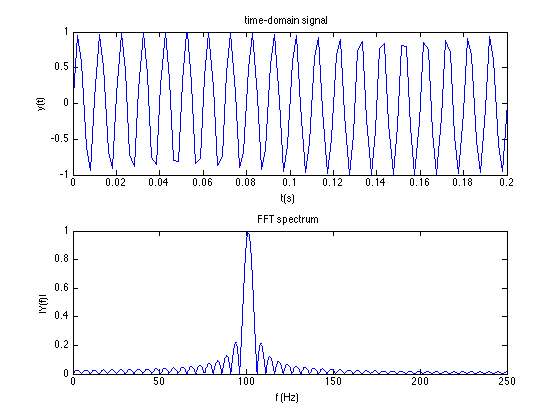
\includegraphics[scale=0.75]{ELEC_1.png}
\caption{FFT Transformation}
\begin{minipage}{0.75\textwidth}
{\footnotesize This is a FFT transformation. As we can see, the dominant frequency is at $100hz$}
\end{minipage}
\end{figure}
\FloatBarrier

\FloatBarrier
\subsection{Full Image}
\begin{figure}[h!]
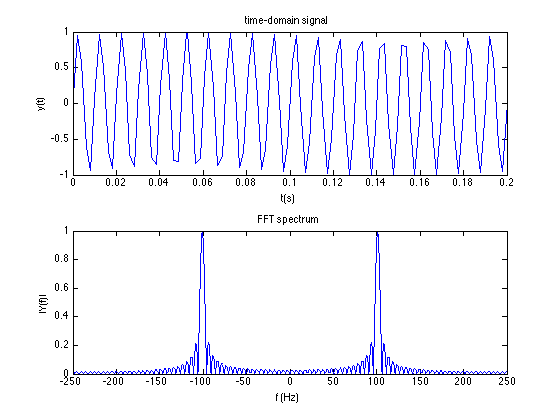
\includegraphics[scale=0.75]{ELEC_2.png}
\caption{FFT Transformation with its mirror image}

\label{img:full}
\begin{minipage}{0.75\textwidth}
{\footnotesize This is a FFT Transformation with its mirror image}
\end{minipage}
\end{figure}
\FloatBarrier
 
As we can see from figure \ref{img:full}, it has its mirror image at the negative frequencies.

\subsection{The relationship}

Below I will use the modification of the \ref{img:original} to demonstrate the relating relationship.

\FloatBarrier
\begin{figure}[h!]
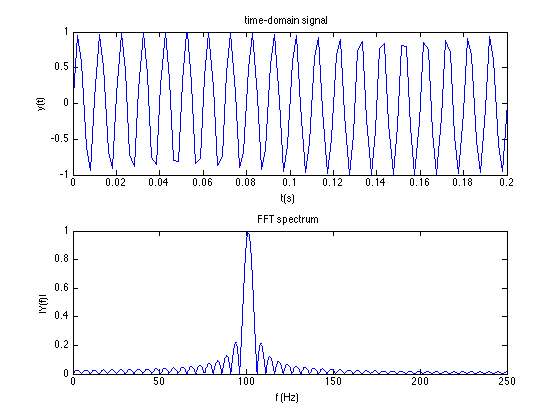
\includegraphics[scale=0.75]{original.png}
\caption{The original picture}

\label{img:original}
\begin{minipage}{0.75\textwidth}
{\footnotesize This is a FFT. The sample rate is at $500hz$. The number of samples points is at 100. The number of FFT sample points is at $2^{18}$}
\end{minipage}
\end{figure}
\FloatBarrier

\begin{enumerate}
\item{Number of FFT points}

Increasing the number of FFT points will result in the increasing of the number of the points in the FFT picture.

\FloatBarrier
\begin{figure}[h!]
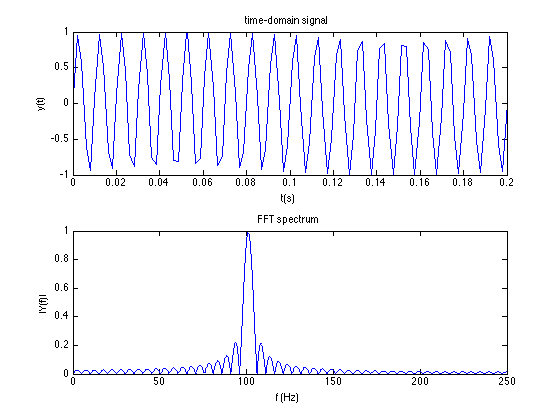
\includegraphics[scale=0.75]{fft_samples_2_20.png}
\caption{Number of FFT points at $2^{20}$}

\label{img:FFT_points}
\begin{minipage}{0.75\textwidth}
{\footnotesize This is a FFT. The number of FFT points changed from $2^{18}$ to $2^{20}$}
\end{minipage}
\end{figure}
\FloatBarrier


\item{Number of samples}

Increasing the number of samples will result in the increasing of the number of the points in the original picture.

And what's more, it will increase the times of plotting period, it is because we use the code like this:
\begin{verbatim}
t = linspace(0,n*Ts,n);
\end{verbatim}

More importantly, it will results in the FFT plots more closer to its theoretical image. The related FFT image will have a shaper peak. 

\FloatBarrier
\begin{figure}[h!]
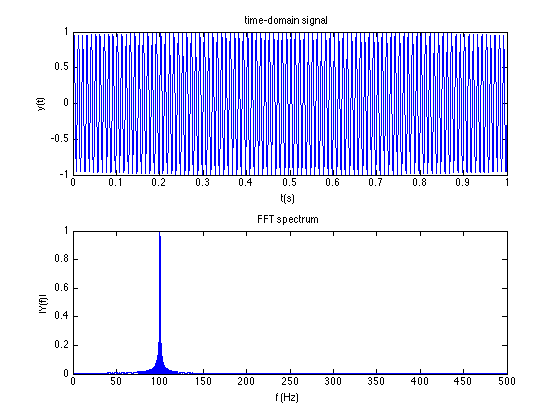
\includegraphics[scale=0.75]{num_of_samples_1000.png}
\caption{Number of samples points at 1000}

\label{img:samples_points}
\begin{minipage}{0.75\textwidth}
{\footnotesize This is a FFT. The number of sample points changed from $100$ to $1000$}
\end{minipage}
\end{figure}
\FloatBarrier

\item{Sample rate}

As we can see from the images above, the FFT picture's frequency domain's length is the sample rate. So it start from $-sample\_rate/2$ and end to $sample\_rate/2$. That also explained why we need the $sample\_rate >= sample\_frequency * 2$

\FloatBarrier
\begin{figure}[h!]
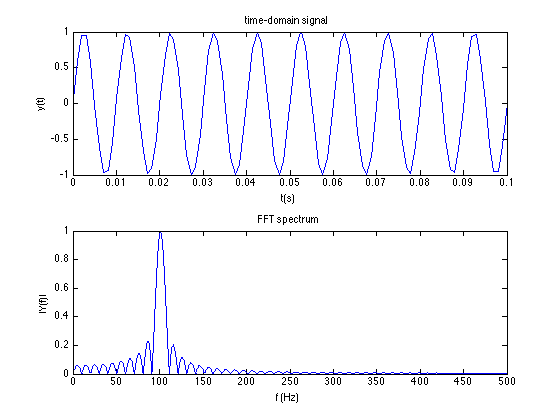
\includegraphics[scale=0.75]{sample_rate_1000.png}
\caption{Sample rate at $1000hz$}

\label{img:sample_rate}
\begin{minipage}{0.75\textwidth}
{\footnotesize This is a FFT I modified the sampling rate from $500hz$ to $1000hz$}
\end{minipage}
\end{figure}
\FloatBarrier
  
\end{enumerate}

\subsection{Noise}
\FloatBarrier
\begin{figure}[h!]
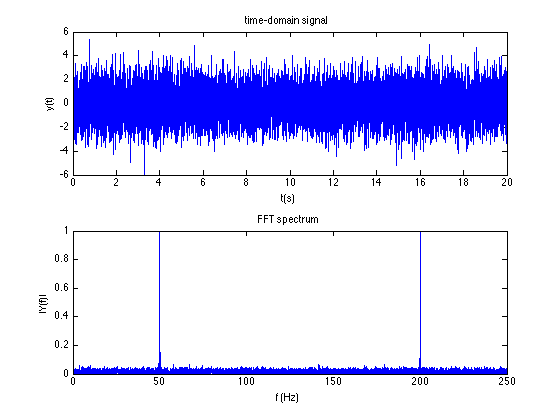
\includegraphics[scale=0.75]{elec_3.png}
\caption{FFT Transformation with noise}

\label{img:noise}
\begin{minipage}{0.75\textwidth}
{\footnotesize This is a FFT Transformation with noise}
\end{minipage}
\end{figure}
\FloatBarrier
As we can see from figure \ref{img:noise}, we can easily figure out the two fundamental frequencies $f=50hz$ and $f=100hz$.

\section{Square wave}

\subsection{Square wave}
\FloatBarrier
\begin{figure}[h!]
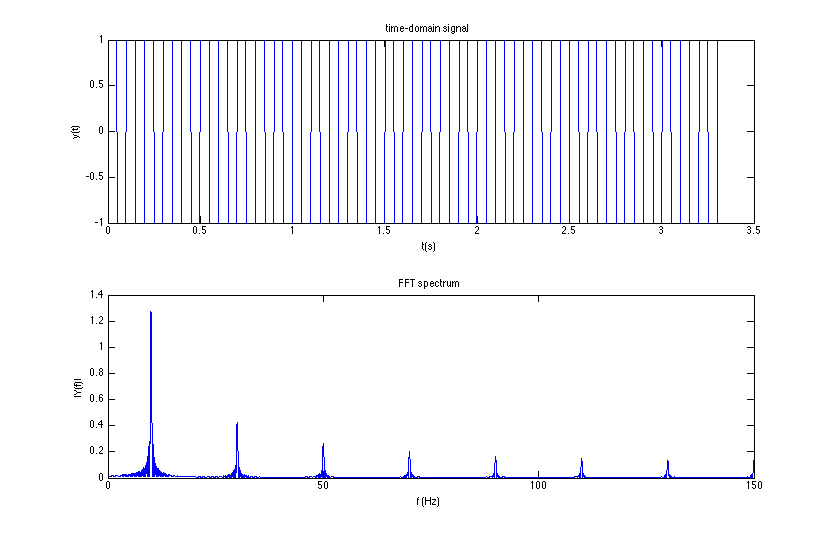
\includegraphics[scale=0.5]{elec_4.png}
\caption{FFT Transformation fore square wave}

\label{img:square}
\begin{minipage}{0.75\textwidth}
{\footnotesize This is a FFT Transformation for square wave}
\end{minipage}
\end{figure}
\FloatBarrier
As we can see from figure \ref{img:square}. This FFT transformation goes infinitely with numerous harmonics. \\

Because it is a square wave, it is composed by infinite frequencies. That is why we have so many harmonics.

The reason why it is "rounded" is because our channel cannot transmit infinite length of frequency. i.e. the bandwidth is at fixed length. So, only the main frequency components are transmitted.  

\subsection{NRZ Noise}

According to the laboratory sheet. We are right now generating the so called NRZ noise. Below are the results, where figure \ref{img:linear} is the picture at linear axis and figure \ref{img:log} is the picture at db axis.

\FloatBarrier
\begin{figure}[!h]
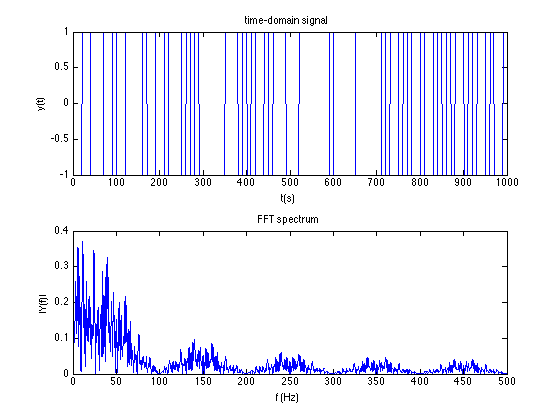
\includegraphics[scale=0.6]{elec_2_1.png}
\caption{ NRZ noise and its Spectrum}

\begin{minipage}{0.75\textwidth}
{\footnotesize Above is the so called "NRZ" noise and below is its spectrum in linear x-axis.}
\end{minipage}
\label{img:linear}
\end{figure}

\begin{figure}[!h]
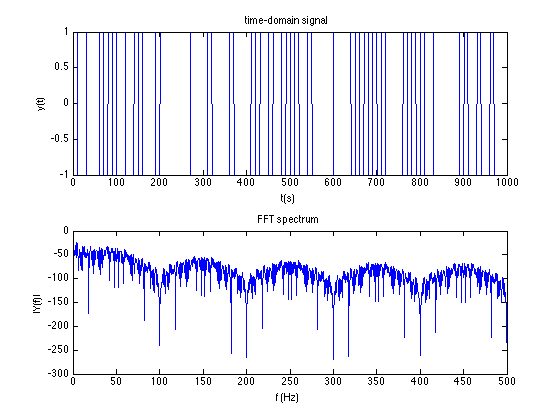
\includegraphics[scale=0.6]{elec_2_2.png}
\caption{ NRZ noise and its Spectrum}

\begin{minipage}{0.75\textwidth}
{\footnotesize Above is the so called "NRZ" noise and below is its spectrum in log x-axis}
\end{minipage}
\label{img:log}
\end{figure}
\FloatBarrier

\begin{enumerate}
\item{frequencies of the nulls in the spectrum}

As we can see from the picture, the frequencies at the nulls are actually integral multiply of the bit rate.
\FloatBarrier
If we change the bit rate to $250 bit/s$. We will get a new picture:

\begin{figure}[!h]
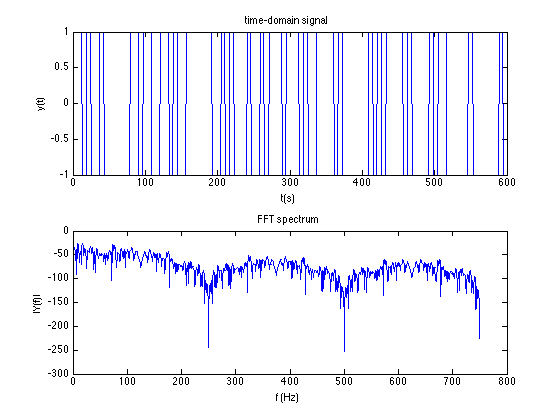
\includegraphics[scale=0.6]{elec_2_3.png}
\caption{ NRZ noise and its Spectrum}

\begin{minipage}{0.75\textwidth}
{\footnotesize Above is the so called "NRZ" noise and below is its spectrum in log x-axis. The bit rate is at $250 bit/s$}
\end{minipage}
\end{figure}
\FloatBarrier

\item{The spectrum}

As we can see from the image, the spectrum for the NRZ noise is in a mass in comparison to the periodical rectangular wave.

That is because the source of our signal was generated from random.

\end{enumerate}



\section{Signal Generator}
\subsection{Sinusoid waveform}
\FloatBarrier
\begin{figure}[!h]
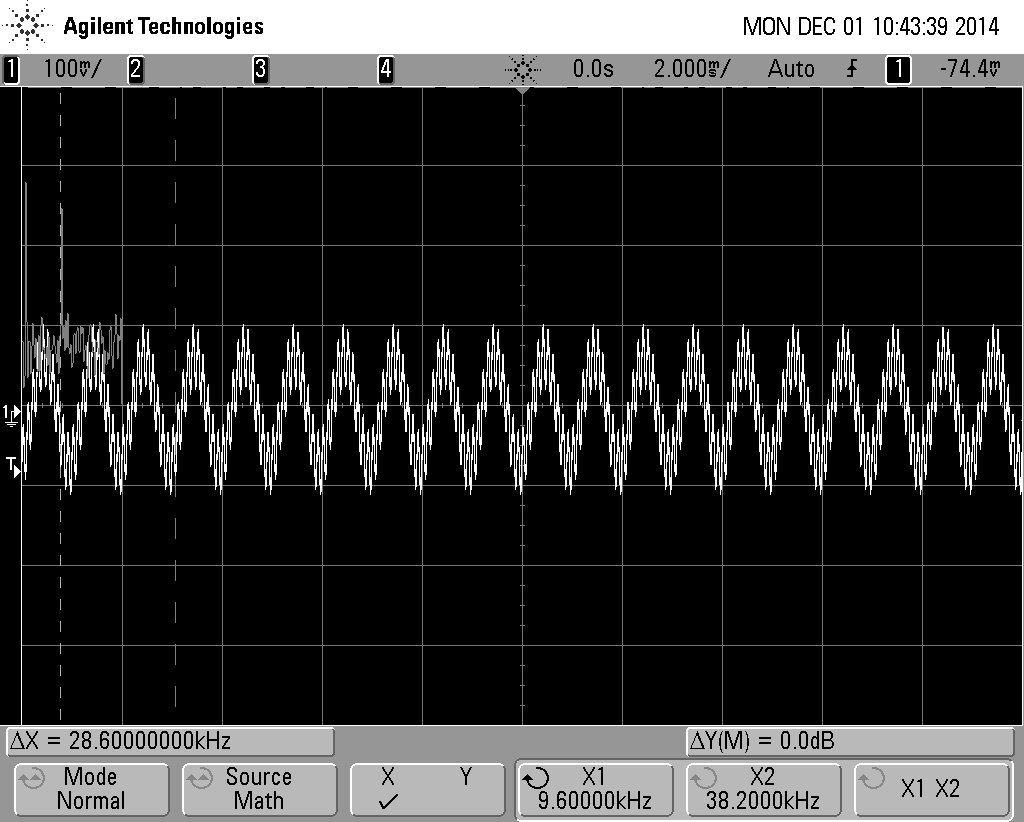
\includegraphics[scale = 0.25]{elec_3_1.png}

\caption{Signal's waveform and its FFT transformation }

\begin{minipage}{0.75\textwidth}
{\footnotesize This is the output of the oscillator for the signal waveform and its FFT transformation}
\end{minipage}
\end{figure}
\FloatBarrier


\subsection{Arbitrary waveform}
It is like we change the Sampling rate in the Matlab. Change the sample rate will result in the FFT be more closer to the theoretical image and will introduce more data in the time domain image by getting a longer period of signal.\\

Blow is the comparsion:

\begin{figure}[!h]
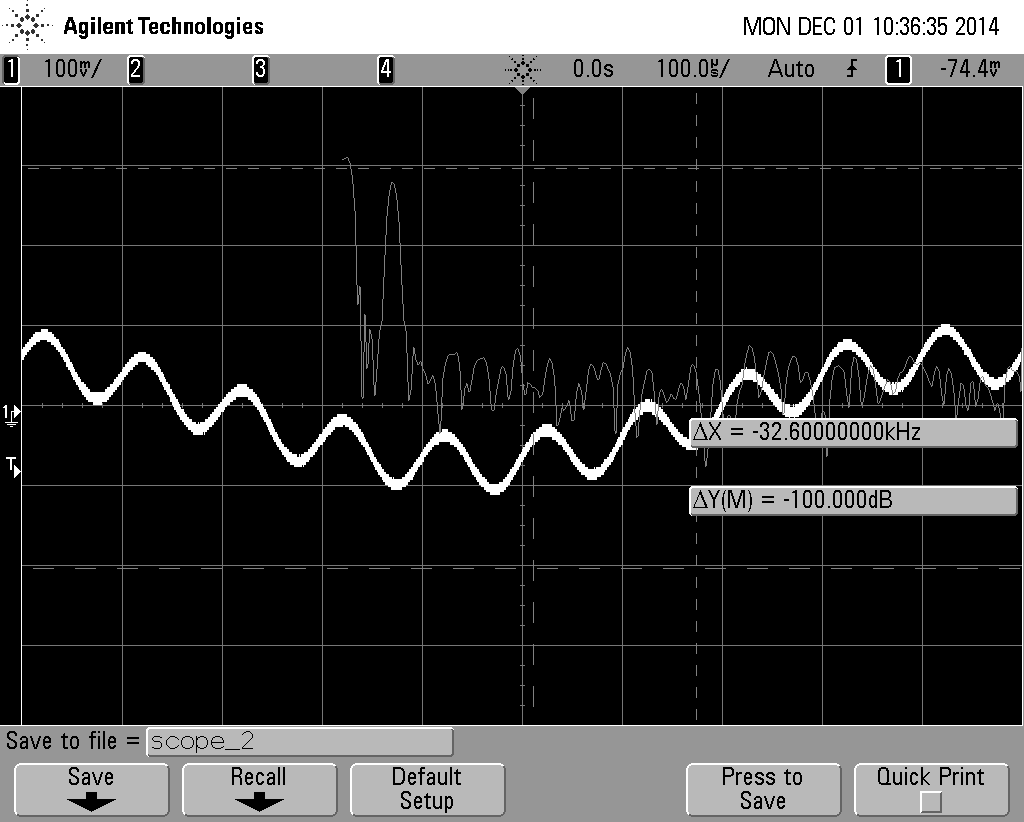
\includegraphics[scale = 0.25]{elec_4_1.png}

\caption{low sample rate}

\begin{minipage}{0.75\textwidth}
{\footnotesize This is a output from oscillator at low sample rate}
\end{minipage}
\end{figure}

\begin{figure}[!h]
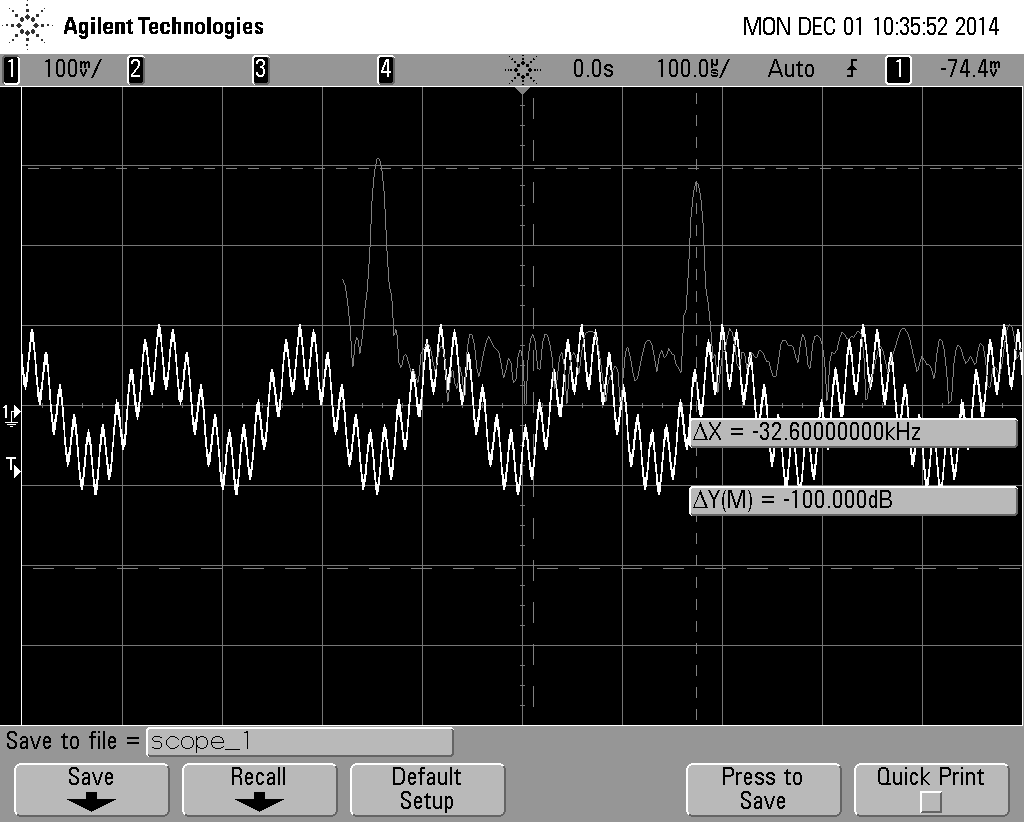
\includegraphics[scale = 0.25]{elec_4_2.png}

\caption{High sample rate }

\begin{minipage}{0.75\textwidth}
{\footnotesize This is the output of the oscillator at higher sample rate }
\end{minipage}
\end{figure}




\end{document}
